\chapter{绪论}
\label{chap:intro}

移动互联网随着智能手机的普及爆发,在智能手机上使用应用成为了日常生活中必不可少的部分,应用几乎涵盖了日常生活的所有部分,衣食住行等等都能通过应用来解决。
正是因为人们对应用的依赖如此之深,应用的安全性成为了各大应用市场需要解决的头号问题。
本章将首先在~\ref{sec:market-overview}节中介绍移动应用市场,然后~\ref{sec:market-prob}节会对应用市场面临的问题进行阐述与分析,最后在~\ref{sec:intro-conclusion}节中,本文将给出的解决方案进行一个大致的描述。

\section{移动应用市场现状}
\label{sec:market-overview}
截止到2016年第三季度, Android系统在全球移动操作系统市场份额中占86.8\%,IOS系统占12.5\%,这两大主流移动操作系统总共占比99.3\%,可以认为是整个市场的全部\footnote{Smartphone OS Market Share, 2016 Q3: \url{http://www.idc.com/prodserv/smartphone-os-market-share.jsp}}。
在腾讯的2016年微信用户数据报告中,截止2016年第一季度,微信月活跃用户达到6.5亿,覆盖200多个国家。
在2016年阿里巴巴双十一活动中,总交易额高达1207亿元,其中无线占比达到81.87\%。
可见移动平台在互联网中占据着重要的位置。
而应用市场作为应用部署到用户设备上的入口,在移动互联网生态闭环中地位尤其重要。

其中IOS系统是由美国苹果公司开发的移动操作系统,只能运行在苹果公司生产的移动设备上,因此IOS的生态圈都由苹果公司主导。
IOS应用分发都通过苹果公司自己运营和审查的App Store进行,App Store预先安装在了每个IOS设备上,开发者通过把应用提交到AppStore,
苹果公司审核通过后用户就可以通过App Store下载安装软件。除此之外还有“PP助手”等第三方应用商店,相比App Store用户量较少。


对于Android市场情况则复杂的多,Android系统由Google公司主导,并且该操作系统持开放的策略,只要符合“开放手机联盟”的标准,任何公司都可以生产运行Android系统的设备。
Android生态圈和IOS生态圈最大的区别是去中心化,Android系统允许用户直接使用软件安装包,因此出现许多应用商店。
在北美以及欧洲地区,由Google公司开发维护的Google Play是最主要也是最权威的Android应用商店,占据了绝大部分用户。
Google Play市场拥有比较严格的应用审查制度,对新上传的应用会进行自动化的程序安全隐私分析以及病毒检测,同时市场对应用提供的内容有分级(类似于电影分级)并且要求应用开发者提供相应的隐私申明等等。
在中国,安卓应用下载存在非常多的渠道,从而也存在着各种各样的应用商店,各自提供不同程度的定制服务(例如推送、应用收费服务、推广服务等)。
然而这也导致中国的Android生态环境异常复杂,市场缺乏统一的、有效的、具有公信力的审查制度。
在中国Android生态环境中,包含了三类应用商店:一是手机厂商的应用商店,通常在用户手机出厂预装的ROM上就安装好了这一类应用商店的入口,其中以“小米应用商店”为代表,其预装在每一台运行MIUI系统的小米手机上,其他非MIUI系统的Android手机用户可以自行安装“小米应用市场”;二是第三方应用商店,通常是互联网公司的一项业务,其中以“360应用市场”和“腾讯应用宝”为代表,用户安装了“360手机助手”就会被引导进入“360应用市场”下载App,安装了微信的用户也都可以通过微信提供的入口进入“腾讯应用宝”;三是运营商的应用商店,通常出现在合约机的预装软件中,由电信运营商开发维护。
中国的人口基数大,得益于良好的基础建设,接入互联网的人数众多,手机应用使用用户量巨大。
如图~\ref{fig:user-scale}所示,根据艾媒咨询《2015-2016中国手机应用商店年度报告》,2015年第四季度共有4.4亿用户在中国使用第三方手机应用商店。
Android的开放策略加上中国的网络环境因素导致了中国异常复杂的Android生态环境,混乱且缺少监管的生态存在许多安全漏洞,应用商店上恶意的Android应用和第三方库给用户的隐私带来非常重大的安全隐患。

\begin{figure}
	\centering
	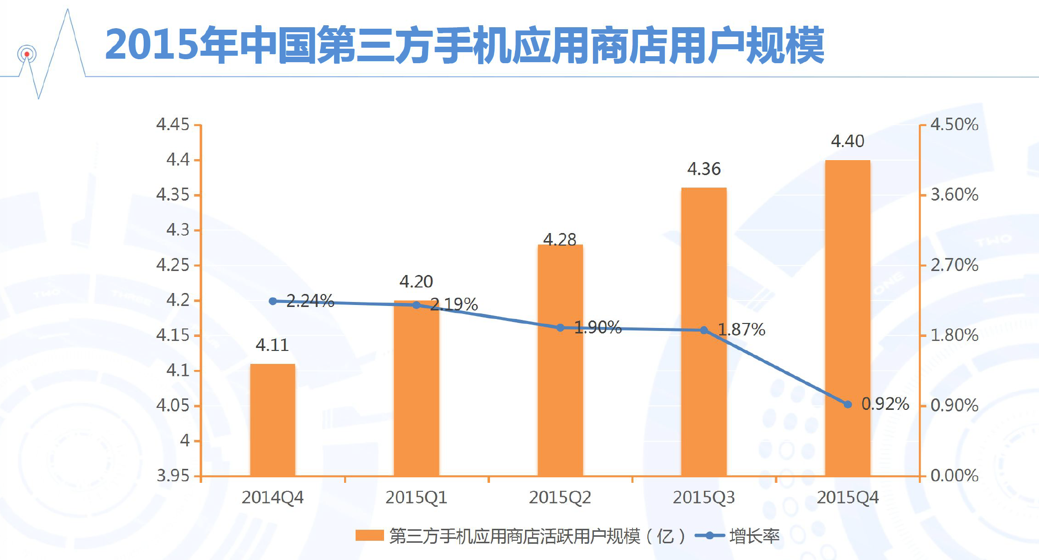
\includegraphics[width=0.9\textwidth]{figure/user-scale.png}
	\bicaption[fig:user-scale]{艾媒咨询《2015-2016中国手机应用商店年度报告》}{艾媒咨询《2015-2016中国手机应用商店年度报告》\protect\footnotemark}{Fig}{Annual Report of China Mobile Application Store}
\end{figure}
\footnotetext{《2015-2016中国手机应用商店年度报告》\url{http://www.iimedia.cn/40366.html}}


\section{面临的问题以及解决方案}
\label{sec:market-prob}
2015年6月,美国网络安全公司NowSecure发布报告称\footnote{新华网:三星手机被曝存安全漏洞 超6亿用户信息存泄漏隐患。 \url{http://news.xinhuanet.com/finance/2015-06/24/c_127945927.htm}},预装在三星Galaxy手机上的SwiftKey输入法在更新后,存在可以被黑客利用的安全漏洞。
被攻击的机器可以允许攻击者控制用户的网络流量,并在手机上留下后门,攻击者可以在手机上执行任意代码。
并且由于SwiftKey为三星预装软件,所以在非root情况下是无法被卸载的。
利用这一漏洞,攻击者可以监控用户的网络,使用受害者手机摄像头、窃听通话等危害用户隐私的行为。
据统计,有超过6亿部三星手机由于该漏洞处于安全威胁之中。


2015年10月19日,苹果公司(由SourceDNA安全公司提供样本)下架了256款App\footnote{新华网:广告公司涉窥隐私 苹果下架众多应用。 \url{http://news.xinhuanet.com/tech/2015-10/20/c_1116881103.htm}},原因是这些App都使用了第三方广告库有米SDK,该SDK调用了IOS系统的私有API获取邮件地址、设备认证信息和路由数据等隐私数据。
根据苹果公司的解释,这些API并不开放给应用使用,有米SDK通过技术手段绕过了App Store的检查,这些使用了有米SDK的应用造成了用户隐私数据的泄露,将无法上架App Store。
由此可见应用的审查对于应用市场是非常必要而且重要的。


中国工信部曾在微博上公布过2015年第三季度问题应用软件名单,其中35款不良应用榜上有名,其中不乏知名大公司千万级用户量的产品,名单上App的主要涉及强行捆绑安装、未经用户同意收集个人信息、恶意“吸费”等问题。

另外,有些违法分子甚至盗用正版应用,并通过技术手段为其增加广告、甚至病毒,最后重新打包发布到应用市场上赚取非法利益。
通过这种技术重打包的应用通常叫做克隆应用。
克隆应用的危害在中国尤其严重。
由于在中国无法使用安卓官方市场Google Play,第三方市场成为了智能手机用户下载应用最主要的方式。
而第三方市场碎片化严重,监管情况不明,导致克隆应用泛滥。
之前研究有对百度应用市场进行检测,12442个应用中有1928个应用为疑似克隆应用,比例超过10\%。可见克隆应用问题情况之严重。

Android的权限机制可以在一定程度缓解恶意应用以及隐私泄露问题。
Android操作系统会在安装应用时告知用户此应用会使用到手机的哪些权限。
比如App需要连接网络或者获取通讯录,开发者要在App中显示申明需要网络权限和读取通讯录的权限。
用户在安装Android App的时候,系统会弹窗描述该App需要获取的权限,用户只有允许才能安装使用。
但是根据相关用户调查,大部分普通用户不会仔细看安装应用时请求的权限。
甚至一些应用商店安装应用时会跳过这个步骤,直接授予App接触敏感信息的权限,由此造成的问题比如一个手电筒应用能够读取用户通讯录的内容非常普遍。
而虽然Android 6.0版本使用了运行时授权, 在应用使用到相对敏感的权限时会提醒用户是否允许应用使用此权限,在一定程度上提高了隐私信息的安全性,但是Android系统版本碎片化严重。
截止2016年5月2日,Android 6.0系统只有7.5\%的装机量,而且动态权限方法无法追踪获取的信息流向,所以并不能完全消除隐私泄露隐患。

市面上有“360手机卫士”,“腾讯手机管家”等工具App查杀Android手机病毒。
通常手机病毒会做些诸如劫持支付软件,记录输入的账号密码,自动发送短信的行为,手机病毒查杀工具可以根据这些行为特征进行静态或者动态的安全保护。

但是这些手机病毒查杀工具对于隐私保护的效果甚微,因为隐私泄露没有明显特征。
例如一个App获取了设备通讯录信息并发送到服务端,查杀工具难以判断这是否是一个恶意的隐私泄露行为,因为诸如微信等App需要通过通讯录信息帮助用户添加好友。
再例如一个App收集用户的手机号码,在发送到服务端的时候不直接将手机号码放在发送的内容中,而是通过发送1次“a”,3次“b”,5次“c”来表示“135”。
这种泄露方式难以发现,Android的用户隐私安全受到了极大的威胁。

以上事例都生动的说明了应用市场需要对开发者上传的应用进行审核。
审核过程包括但不仅限于查杀病毒、分析应用是否具有恶意行为以及检查克隆应用等等。
在进行单应用审计的同时,应用市场还可以综合海量的审计结果,进行分析与预警。
之前轰动一时的XcodeGhost,就是在编译iOS App时向应用代码中注入了恶意的代码,使得App运行是会收集用户的信息并且上传到攻击者的服务器;
之前在研究中发现很多病毒也会伪装成正常的包名来躲避安全分析工具的检查,例如病毒DroidKungFu~\supercite{kungfu}就是在感染的app中伪装成\texttt{com.google.update}(Google的应用更新服务库)。
只要应用市场能够实时监控与分析海量的审计结果,上述病毒的爆发就能即使被发现并制止。

在应用开发中,通常会使用到第三方库。
第三方库为开发者提供一个或一组编写好的功能,加速软件开发。
研究表明第三方库的质量参差不齐,很多广告库会泄露用户的隐私,而最近发生的淘米客和百度SDK事件则更加恶劣,这些SDK中嵌入了远程命令和控制服务器(C\&C服务器),使得目标机器可以接受来自服务器的命令,从而被控制,给外界提供传输恶意命令的平台,危害用户的隐私数据安全。
即便没有恶意,很多第三方库还会存在很多漏洞,这些漏洞也可能将用户的手机暴露在不安全的环境中。
同时使用一些可能导致性能问题的第三方库对应用开发者来说也会造成不小的损失。
所以应用市场可以通过检测应用中是否存在有问题的第三方库,来定位问题库的受害者,并提醒开发者使用经过补丁升级后的第三方库,或者禁止使用有问题的第三方库。

综上所述目前第三方应用市场对应用的审查与分析还比较有限,主要体现在以下三个方面:隐私问题审核、重打包应用检测以及第三方库检测。
本文设计的应用审核系统AppShield旨在提供以上功能的同时保证一定的扩展性,使得应用市场能够更加安全,有效。

针对隐私问题审核,AppShield集成了单应用审查工具AppAudit~\supercite{appaudit},对于单个应用,会使用AppAudit进行分析,检测出隐私泄露威胁;
同时AppShield会结合整个市场的应用检测结果进行进一步分析,得出市场的隐私泄露概要,以及市场上造成隐私问题最多的组件,并对其进行深度分析。

针对重打包应用和第三方库检测,AppShield设计了一种应用相似度检测的方法,可以同时应用与以上两种检测中。
对于每个应用,此方法会进行一次指纹提取,生成应用的指纹信息;
依据指纹信息进行比对,可以得出应用之间的相似度,从而找出潜在的重打包应用;
由于相似度检测的方法是基于应用代码的,所以第三方库可以使用dex工具打包成SDK,通过比对此SDK和应用的相似度,即可知道应用是否包含了这个第三方库。

在检测应用相似度的工作上,最大的挑战就是混淆。
而AppShield中使用的方法能够应对大多数情况的混淆方法,使得系统能够检测出使用了混淆技术的重打包应用,使得检测的广度得到了提高。

\section{本章小结}
\label{sec:intro-conclusion}
本章首先介绍了移动市场繁荣的现状,然后对目前应用市场存在的问题进行了分析与讨论,最后提出了应用市场需要有检测隐私泄露问题、检测重打包应用、检测第三方库三方面的能力,并给出了AppShield解决方案,同时阐述了AppShield多方面的优点。